\documentclass[11pt,a4paper]{article}

\usepackage[T1]{fontenc}
\usepackage{mathptmx}
\usepackage[margin=2.2cm]{geometry}
\usepackage{microtype}
\usepackage{graphicx}
\usepackage{caption}
\captionsetup{font=small,labelfont=bf}

\setlength{\parskip}{0.5em}
\setlength{\parindent}{0pt}
\pagestyle{empty}
\renewcommand{\topfraction}{0.9}
\renewcommand{\bottomfraction}{0.8}
\renewcommand{\textfraction}{0.1}
\renewcommand{\floatpagefraction}{0.8}
\setcounter{totalnumber}{4}

\begin{document}

{\large\textbf{Dense versus CSR inference of pruned Qwen2.5-0.5B on CPU}}\\[0.2em]
Zihang Peng, October 2026 \hfill First iteration, short report

\medskip

\textbf{Question.} The goal of this first iteration was simple. If we prune
a small language model, at what sparsity does running its layers in a
sparse format (CSR) become faster than running them dense, and is the model
still good at that sparsity? I also wanted to understand why CSR is fast or
slow, so that the next steps start from real numbers.

\textbf{Setup.} I used Qwen2.5-0.5B and PyTorch on CPU, as you suggested.
PyTorch lets me replace selected Linear layers by CSR layers and keep the
rest of the model unchanged, so dense and CSR run in the same engine. The
dense layers use oneDNN and the CSR layers use oneMKL; I checked with
\texttt{perf} that both libraries are really called. All runs use fp32, 16
cores of one NUMA node of a Xeon Platinum 8352Y on FinisTerrae~III, and the
whole socket is reserved so that no other job disturbs the measurements.
I pruned the 168 Linear layers of the Transformer blocks with magnitude
pruning, Wanda and SparseGPT, at 30 to 90\% sparsity, and also with N:M
patterns (2:4, 4:8, 1:4) and with $4\times4$ and $16\times16$ blocks. Model
quality is the WikiText-2 perplexity. Code, configuration and results are in
my repository with pinned versions.

\textbf{Quality.} The dense model has a perplexity of 13.1. SparseGPT is
the best method: 13.7 at 30\% sparsity, 17.7 at 50\% and 34 at 60\%. After
that the model breaks down (219 at 70\%). Wanda is a little worse (23 at
50\%) and magnitude pruning already fails at 50\% (481). With the 2:4
pattern SparseGPT reaches 28, and block pruning destroys the model already
at 50\%. So for this model the useful range is up to about 50--60\%
sparsity.

\textbf{Making the comparison fair.} My first CSR version was slower than
it needed to be, and fixing this took a good part of the work. PyTorch
stores CSR indices as 64-bit integers, but oneMKL wants 32-bit integers, so
every call converted the whole index arrays. Using 32-bit indices made CSR
decoding 17--53\% faster. A second problem is the data layout: oneMKL can
only put the sparse matrix on the left, so the activations have to be
transposed, and the transposes cost time. Keeping the MLP block in a
transposed layout helped a little (up to 7\%). Finally, the default
Hugging Face code computes the output logits for every prompt token, which
real inference does not do, so I compute them only for the last token.
Dense timings also vary between nodes and processes, so I always compare
dense and CSR in the same process and take the median of three runs.

\textbf{Main result.} With these fixes, CSR decoding (one token at a time)
becomes faster than dense at about 70\% sparsity and is 1.4 times faster at
90\%. Processing a prompt of 128 tokens needs about 80\% sparsity to break
even, and a prompt of 512 tokens is still slower with CSR even at 90\%
(0.86 times the dense speed). Figure~\ref{fig:gap} shows this next to the quality results, and gives
the main finding: the sparsity
where the model is still good (up to 50--60\%) and the sparsity where CSR
is faster (70\% and more) do not overlap. At 50\% sparsity CSR decoding
runs at only 0.82 times the dense speed. The gain is also limited because
the output layer, about a quarter of the model, stays dense.

\begin{figure}[!htb]
\centering
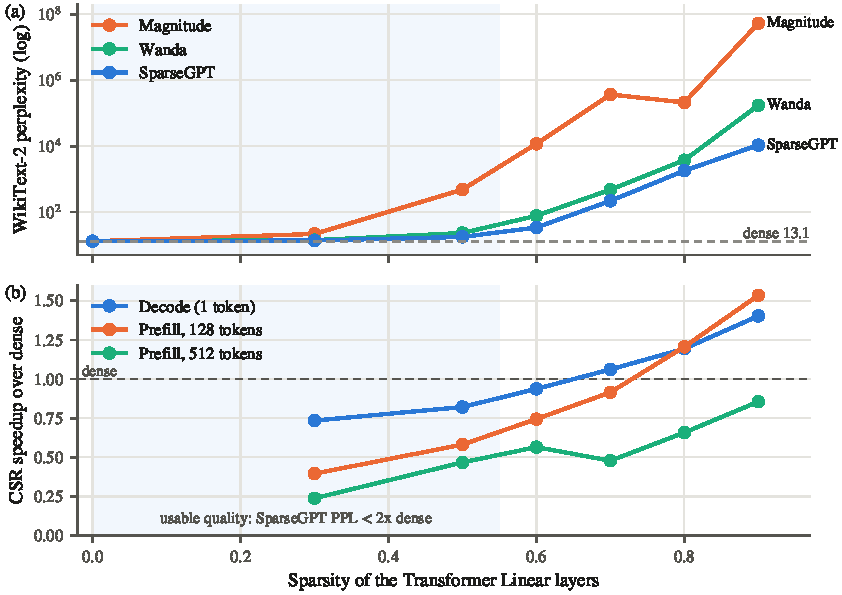
\includegraphics[width=0.78\linewidth]{figures/quality_speed.pdf}
\caption{(a) Perplexity against sparsity. (b) Speed of CSR relative to
dense for the SparseGPT models, with the MLP layers in CSR. Above the
dashed line CSR is faster. The shaded range is where the model keeps less
than twice the dense perplexity.}
\label{fig:gap}
\end{figure}

\textbf{The role of the batch size.} Measuring single layers showed that
the number of rows in the activation matrix (one row when decoding, many
rows when processing a prompt) matters as much as the sparsity. Figure~\ref{fig:rows} shows this for single layers. With few
rows (8 to 32) CSR is already faster than dense at 50\% sparsity, but with
512 rows it needs about 85\%, because dense code reuses each weight much
better when there are many rows. I also learned that single-layer
benchmarks must use a cold cache: one layer fits into the 48\,MB L3 cache,
which makes dense look much better than it is in the full model.

\begin{figure}[!htb]
\centering
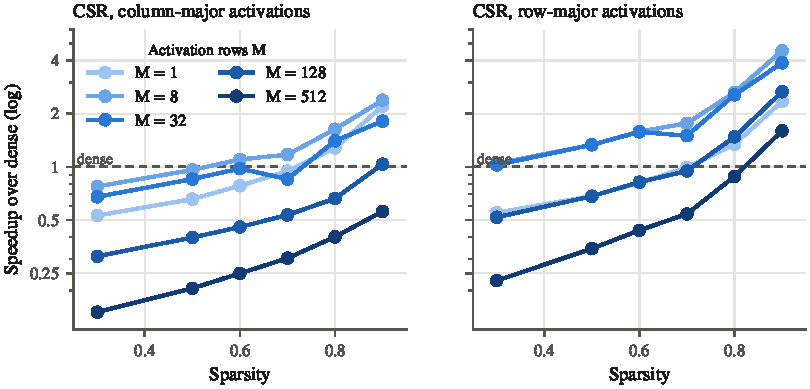
\includegraphics[width=0.85\linewidth]{figures/layers_cold.pdf}
\caption{Speed of CSR relative to dense for single layers with a cold
cache, for different numbers of activation rows $M$ ($M=1$ is decoding).
Left: activations in their normal layout. Right: transposed activations,
which let oneMKL use its faster kernel.}
\label{fig:rows}
\end{figure}

\textbf{The role of the sparsity pattern.} At the same sparsity, the
pattern of the zeros makes almost no difference to CSR. Unstructured, 2:4,
4:8 and block-sparse matrices run at the same speed as a matrix with the
same number of nonzeros at random positions. CSR simply does not use the
structure that pruning creates.

\textbf{Why CSR is slow.} The PyTorch profiler and a Top-down
Microarchitecture Analysis with \texttt{perf} give a clear picture. The
dense kernel either waits for memory (one row) or does useful work most of
the time (many rows). The CSR kernel is not limited by memory bandwidth.
It is limited by the work it does for every nonzero: it loads an index,
loads the matching input value from a scattered position and runs a short
loop whose length changes from row to row. At 50\% sparsity it executes
about 25 times more instructions than the dense kernel for half of the
arithmetic. On top of this, the transposes around the oneMKL call still take
about 16\% of the time when processing a prompt.

\textbf{What this means for the next steps.} The results fit the
directions we discussed. First, a format that uses the structure of the
zeros, such as UZP, could reduce the work per nonzero, and the N:M and
block models from this sweep are ready to test it. Second, the best format
depends on the layer, the sparsity and the number of rows, so a simple rule
could choose dense or sparse per layer and per phase (sparse for decoding,
dense for long prompts). Third, pruning could be made aware of the format,
looking for a pattern between unstructured and block pruning that keeps
the quality but is faster to run. Before that I would like to prune layer
by layer as the original Wanda and SparseGPT code does, check the TMA
numbers with VTune, and look for a way to avoid the transposes. I would be
glad to hear which direction you find most promising.

\end{document}
